\documentclass{tstextbook}

\begin{document}

\tsbook{Game of Physics游戏策划}
       {Game of Physics小组}
       {Cover Designer}
       {2017}
       {xxxxx}{xxx--xx--xxxx--xx--x}{0.0}
%       {Publisher}
       {余方$\ $周诗蕙$\ $张元一$\ $张冰煜}

%---------------------------------------------------------------------------
% Chapters
%---------------------------------------------------------------------------

%---------------------------------------------------------------------------
\chapter{游戏概述}

\begin{summary}
  Game of Physics (游戏名暂定为《物$|$理》)是一个以开放世界、解谜、RPG和沙盒为主要元素,以物理学为背景,美术风格极简,主要面向14-30岁青年玩家的开放世界解谜类3d游戏。
\end{summary}

\section{游戏运行环境}

游戏主体为exe格式(也可同样的源项目在unity中build成适配于mac系统的dmg格式),运行于PC端,Windows或MacOS环境中。在今后成功做出PC端游戏之后,我们也可能考虑推出手游版本。但是在目前,我们先出PC端。

游戏构架在Unity引擎上,以$C\#$为主要语言编写。

\section{游戏故事情节}

游戏分为实验和理论两个模块。在实验模块,游戏将带领玩家领略真实而丰富的物理世界。以经典力学部分为例,随着游戏的进展,玩家将解锁小球、滑块、不同刚体、陀螺等多个角色,获得绳、链、滑轮等多种道具,可将多个角色组合在地图中,形成多角色RPG扮演,在开放世界地图中探索物理规律之神奇。在这一部分,我们的地图将分为经典地图和沙盒自建地图两块。经典地图将还原物理学史上的种种精彩和经典的实验、思想实验,它是解谜和探索的主线,将撑起游戏的整个主体故事。同时玩家还可以在设定好的地图之外自建地图,玩出超高自由度的沙盒玩法。

物理学是一位用理论和实验两条腿走路的巨人。随着实验的进展,玩家将需要探索物理学理论,以进一步解锁物理世界的大地图。玩家将在探索中获取一步步解锁物理理论的必要工具:数学知识,并籍此习得新技能。技能将可以在理论推理中直接使用,因而当你发现推不下去了的时候,就有可能是缺少技能哦!

随着玩家探索和解谜、推理的进行,玩家将不断解锁原先未知的物理世界。在游戏界面右下角的“物理学地图”中,玩家将拨开云雾,逐渐解锁、点亮物理世界的大地图。在“物理学地图”中,玩家可以通过点击地图中的区域,直接传送到已解锁地图中的某一区域中。



\section{游戏特征}

\subsection{游戏目标}

游戏目标在于探索完物理学大地图。在实验模块中,玩家为了得到预期的实验结果和解锁新实验而自发地思考、规划、克服困难。玩家还会在实验模块的沙盒地图中尽情发挥创造力,创造新奇、有趣、丰富多彩的物理系统。在理论模块中,玩家为了解锁新的物理理论,一步步开拓未知、探索真理而主动地推理公式,并且为了学习新技能而学习必要的数学知识。

\subsection{游戏规则}

游戏中的解谜有一套详尽的逻辑关系网。在精致的安排下,玩家在实验模块下完成某一实验、达到某个预期的实验结果后,将会解锁下一个实验,或者理论模块的icons——灵感小灯泡亮起,提醒玩家有某一物理定律可以解锁。

完成某一实验的条件是达到预期实验结果。为此,我们将对所有实验地图设定成功条件,满足成功条件视为实验成功。

解锁某一理论的条件是推理出这项理论(物理学定律、定理、公式等)。由于推理步骤是按照“技能”来的,即,使用某项数学技能后,会推理至相应的结果,故而数学过程不会存在问题。这样,只要最终结果正确(符合预期),即视为推理成功、理论解锁。

解锁新技能的条件穿插在整个游戏里,依游戏剧情所恰当安排。比如觉得玩到哪里,接下来可以学习微积分了,就在这里将“微积分”技能从“不可见”解锁为“可学习”状态;玩到哪里,接下来必须要微积分的知识了,就在这里要求玩家必须解锁“微积分”技能才能继续。学习数学技能的过程可以设置为一个子关卡、子地图,也可以通过穿插在游戏中的CG展现。

\subsection{反馈系统}

游戏将通过以下反馈系统调动玩家的积极性:

\begin{enumerate}
\item{技能树}

技能是必要的数学知识。如微积分、线性代数、傅里叶变换等等。当游戏进行到解锁相关内容,玩家习得这项技能后,这项技能将在技能树中被点亮,并可直接在接下来的游戏中使用。技能树和技能点将增进玩家的成就感。

\item{物理学大地图}

物理学大地图是一张包含物理学所有内容的地图,类似下图\ref{Fig.map}。但我们会手工重新绘制。玩家每解锁一部分主线内容,将在物理学大地图中显示出来。如图\ref{mapUnlock}。(当然肯定要比这张图精致)

\begin{figure}[H]
\centering 
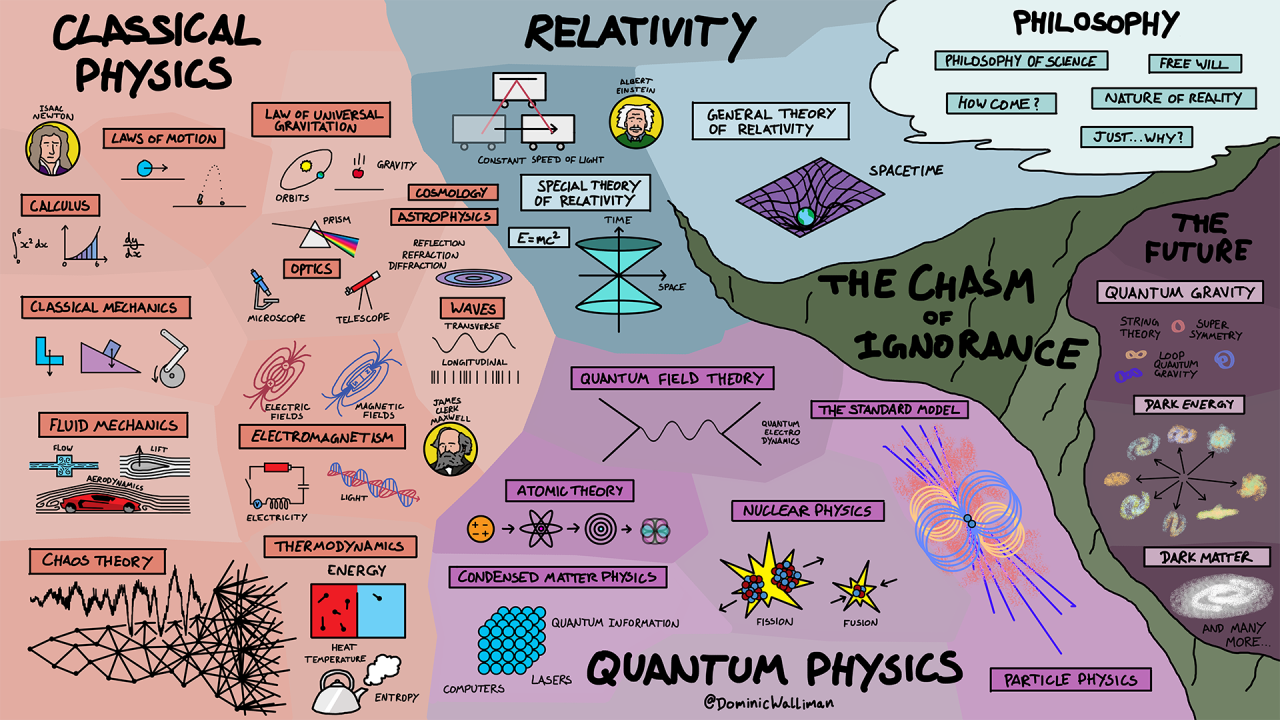
\includegraphics[width=1\textwidth]{MapofPhysics} 
\caption{Map of Physics} 
\label{Fig.map} 
\end{figure}

\begin{figure}[H]
\centering
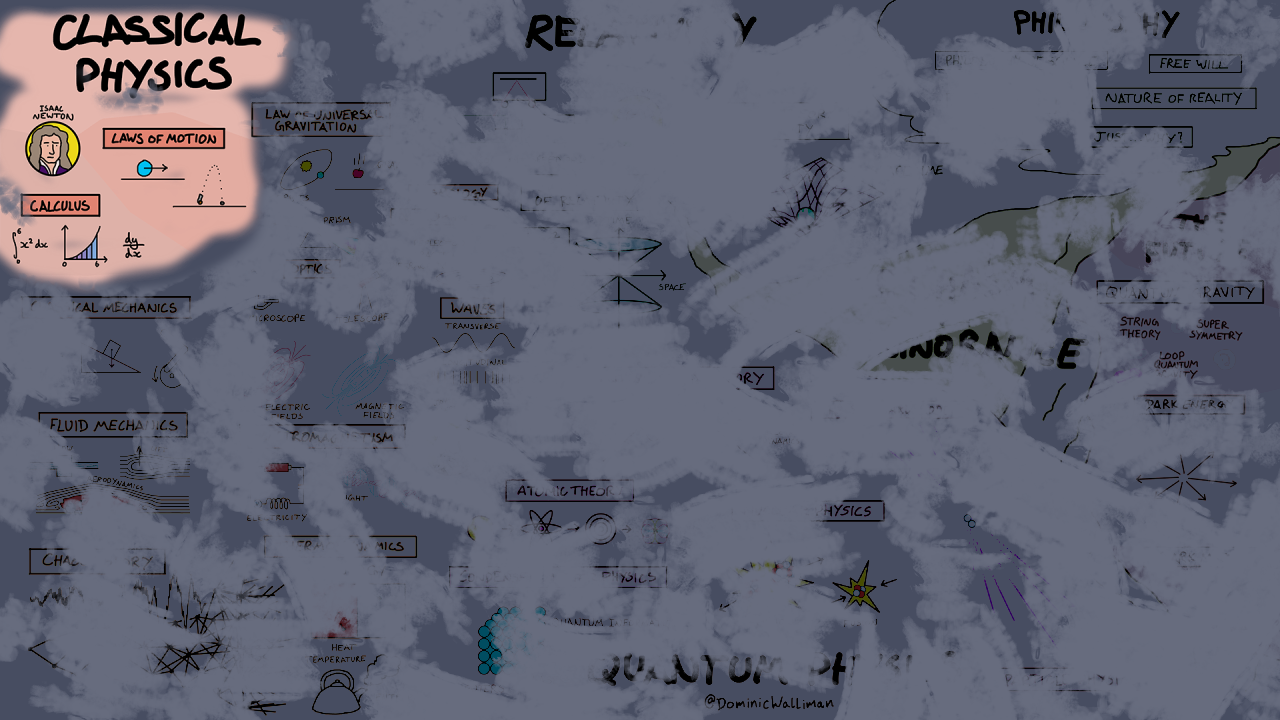
\includegraphics[width=1\textwidth]{UnlockMap} 
\caption{Unlocked Map}
\label{mapUnlock} 
\end{figure}

\item{角色、道具、物品收集}

游戏中,玩家将随着故事的进展逐步解锁不同的角色,如经典力学部分有小球、滑块、杠杆、各种刚体、陀螺等等。这些角色将被玩家永久收入囊中,并且在当前场景里最多可以携带5个角色,以在场景中放置、运动,形成多角色RPG游戏模式。游戏界面的左下角将显示当前场景下的角色信息和状态。

玩家还会随着游戏的进展获得各种道具。这些道具中有用于搭建和组合实验系统的,如绳、链、滑轮等等;也有测量道具和实验仪器,如测速仪、测力计等等。这些道具将被玩家永久收入囊中。在当前场景下,玩家可以随身携带一些道具在界面下方的道具槽中,以随时取用。(类似minecraft中玩家放置一部分道具在场景下方的道具槽中,玩的时候点一下就在当前场景下使用该道具。)

游戏中还会掉落一些物品。这些物品其中一些是彩蛋。见后文。其他类型的物品暂时还没想好。


\item{理论与成就}

已解锁的理论是玩家通过自己的努力解锁的,他们不是教科书上白纸黑字的死的知识,而是玩家自己的发现、自己的推理所获、自己的成就。这将增进玩家的成就感、主动参与感与获得感。

我们可以把重要的理论milestone制作的精美,像宝藏或者勋章,以增强玩家的成就感与获得感。

\item{沙盒与个性化的地图生成}

在实验模块的整个地图中,除了主线故事必有的设计好的地图外,玩家可以使用自己背包里的道具,在周围空白地图中建造自己的实验装置、实验系统,体验沙盒模式的乐趣。建造好的实验装置将保留在玩家的地图中,成为玩家的个性化定制。玩家可以鸟瞰自己目前的地图,尽收眼底的是满满的成就感!

\item{彩蛋$\&$物理背后的故事}

我们会在游戏中穿插一些彩蛋,讲述游戏背后的物理学史上的故事,或致敬物理学上的经典梗(如薛定谔的猫、麦克斯韦妖等等)。彩蛋会并入收集系统,并且提交给steam。玩家之间可以比一比谁收集到的彩蛋多!

\end{enumerate}


\subsection{主动参与}

开放世界的游戏机制将吸引玩家主动参与到探索未知的物理世界中去。

理论模块的解谜和推理的游戏机制将吸引玩家主动探索物理学规律。

游戏的反馈系统将增进玩家的成就感,吸引玩家主动玩下去。

RPG和沙盒模式进一步增加游戏的趣味。

\section{游戏定位}

虽然《物$|$理》以真实的物理科学为背景,希望玩家通过游戏探索和学习物理知识,但是绝不能认为“《物$|$理》是一款教育游戏”而忽视了游戏属性。相反,游戏性必须是《物$|$理》要考虑的重要因素。《物$|$理》是一款游戏,那么它就必须在游戏市场中竞争,它就必须是一款能吸引玩家积极主动投入其中的好游戏。正如某位知乎上的游戏类答主曾说过:“愿世上再没有‘严肃游戏’。”一个好的游戏,不应该通过游戏以外的东西来卖座,来掩饰自己在游戏性上的短板。

游戏的玩家市场定位于14-30岁的年轻人。由于玩家基础的不同,游戏将设置“简单”、“普通”、“困难”和“地狱”四种模式。更难的游戏难度体现在主线要求完成的内容更多、更复杂的实验设计,以及在理论和实验两个模块下均更少的引导和提示上。

我们预计玩家将花5-10小时通关经典力学部分的主线内容。玩家可投入更多时间于更复杂的支线内容、以及沙盒建造中。

\section{游戏风格}

游戏主打极简风格。在极简而审美在线的美术设计中,玩家将免去杂乱元素的干扰,沉浸于物理之美中。同时,极简的风格,搭配上合适、有氛围感的背景音乐,将潜移默化中引导玩家的专注力,使得玩家在行云流水的解谜安排中有沉浸、专注、充满氛围感而丝滑的游戏体验。

\begin{figure}[H]
\centering
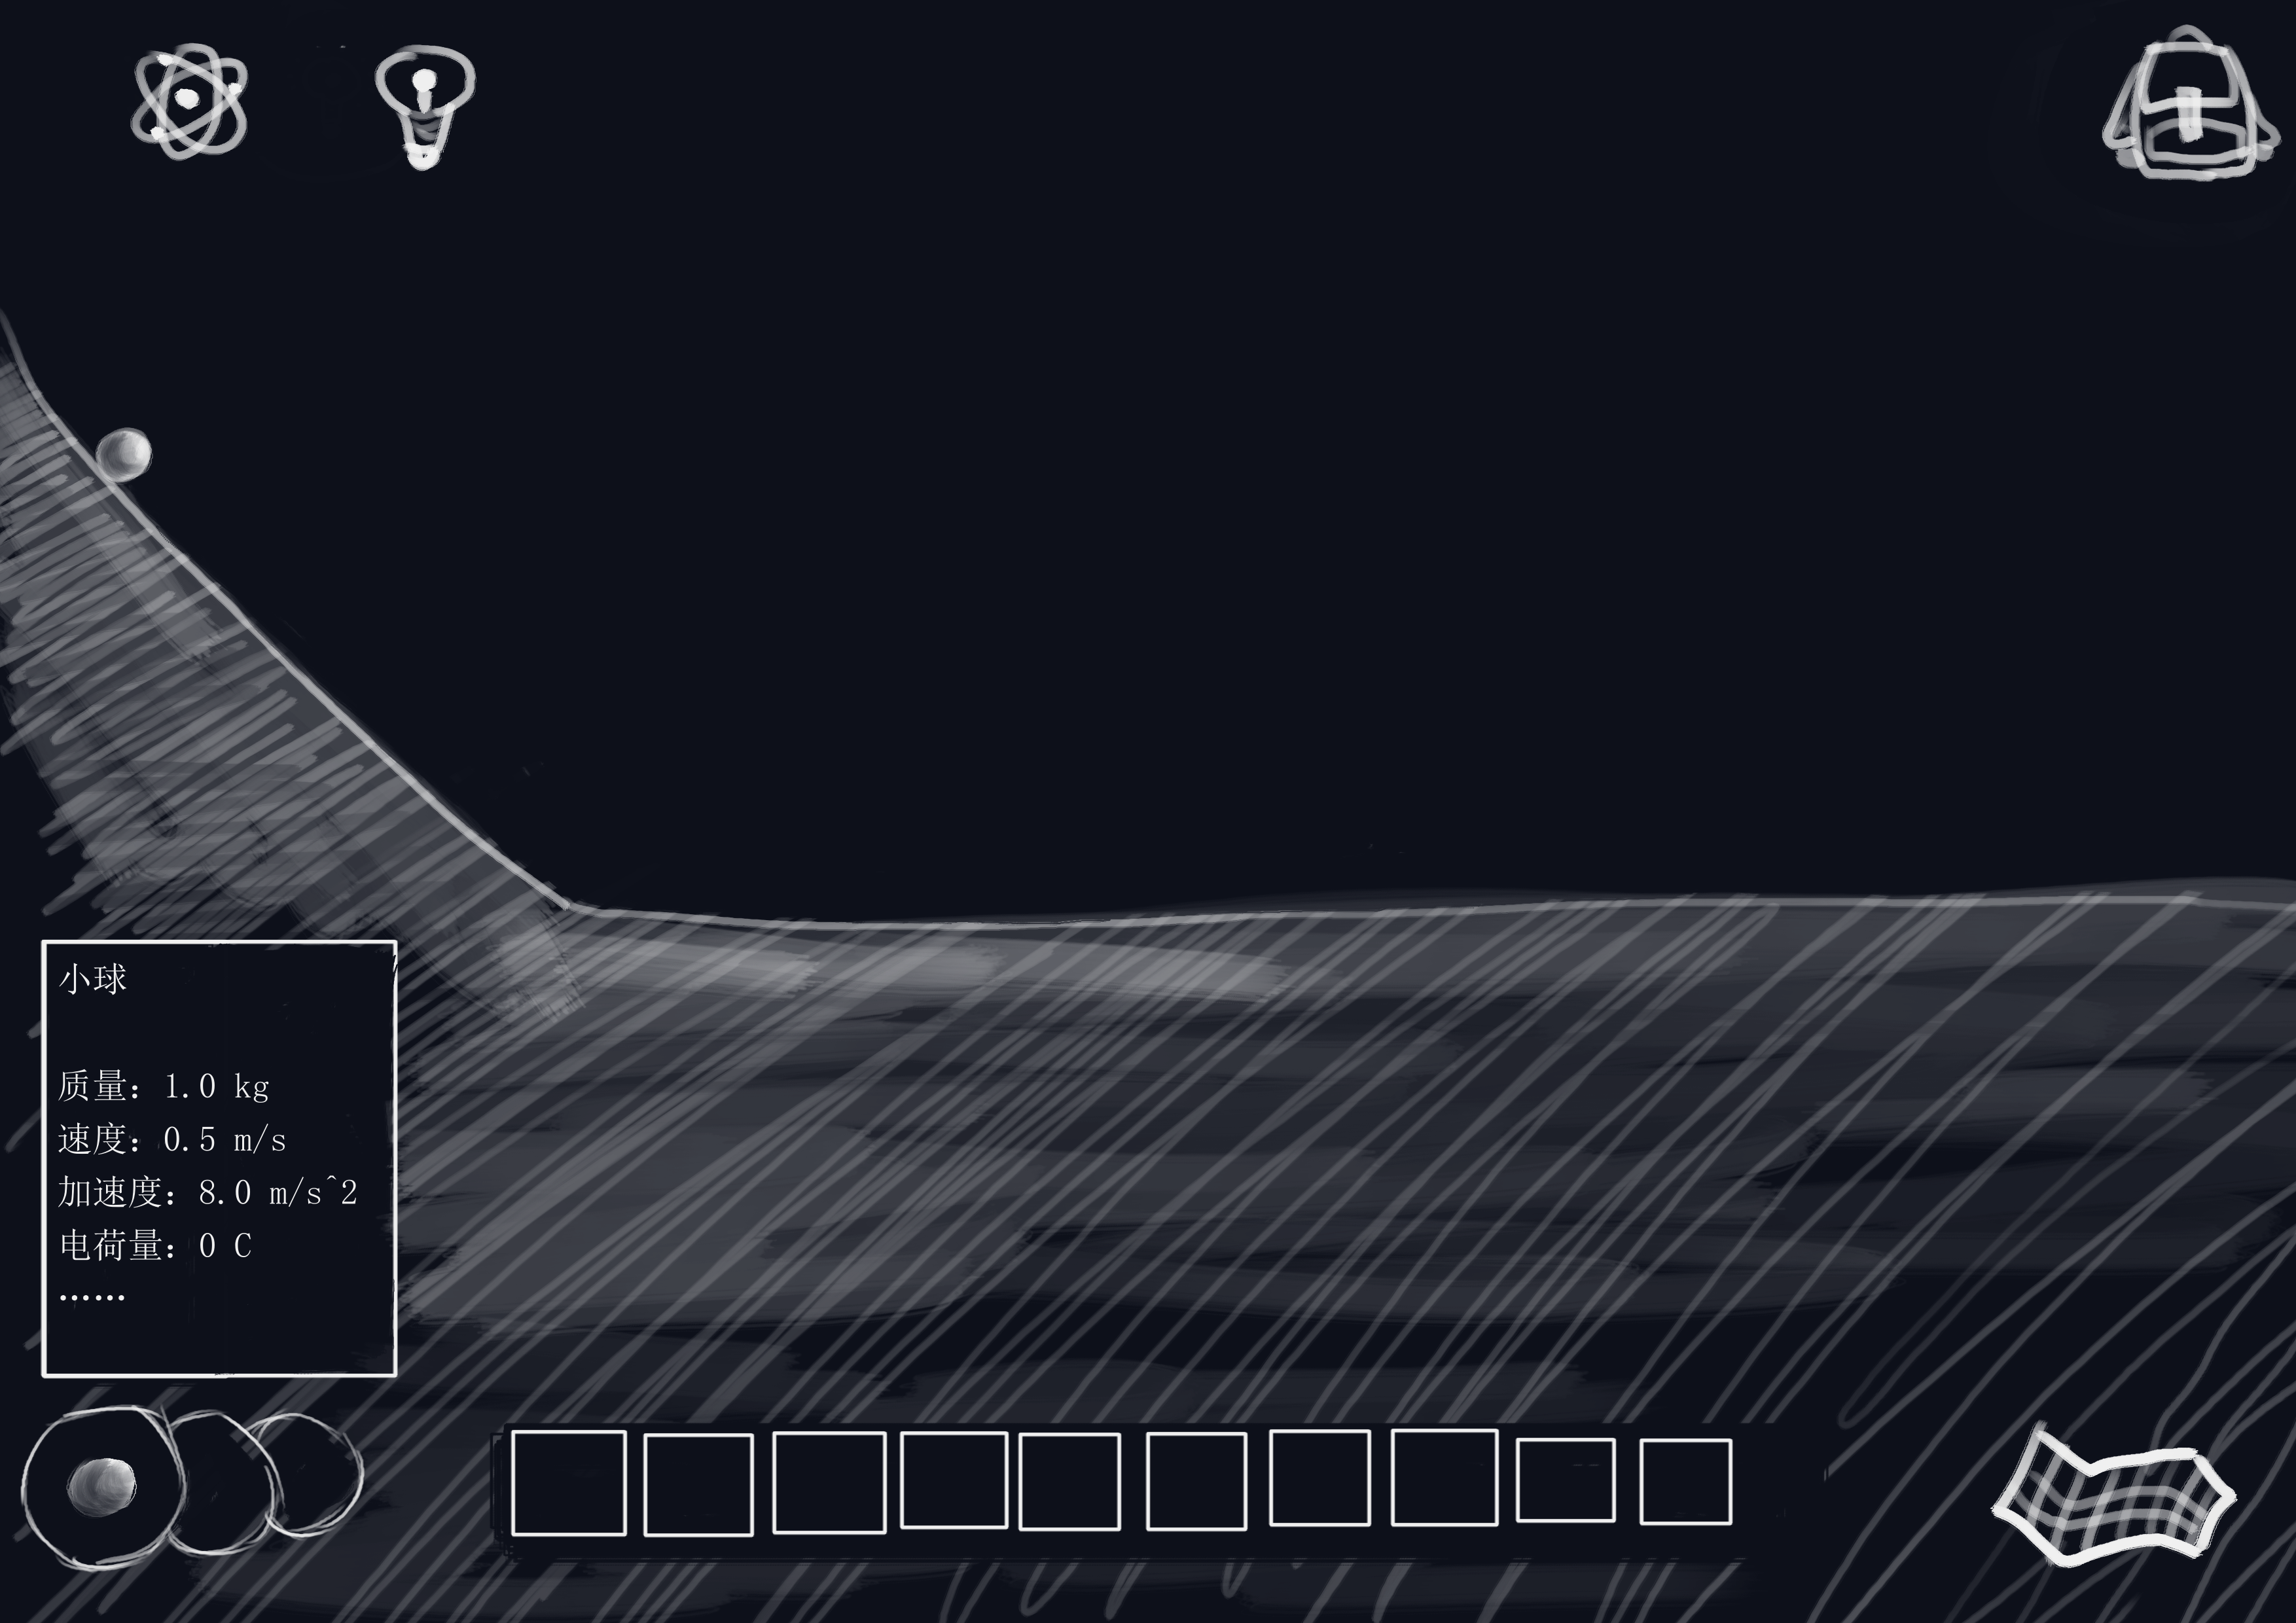
\includegraphics[width=1\textwidth]{MainScene} 
\caption{游戏界面概念图}
\label{MainScene}
\end{figure}

%---------------------------------------------------------------------------
\chapter{游戏机制}

\begin{summary}
《物$|$理》融合了开放世界、解谜、RPG和沙盒机制。
\end{summary}

\section{游戏性设计}


\section{游戏操作}


\section{用户界面}



\section{玩家交互}


%---------------------------------------------------------------------------
\chapter{游戏元素}

\begin{summary}

\end{summary}

\section{角色}


\section{道具}


\section{技能}

%---------------------------------------------------------------------------
\chapter{游戏的故事背景}

\begin{summary}

\end{summary}

%---------------------------------------------------------------------------
\chapter{游戏过程}

\begin{summary}

\end{summary}

%---------------------------------------------------------------------------
% Bibliography
%---------------------------------------------------------------------------

\addcontentsline{toc}{chapter}{\textcolor{tssteelblue}{Literature}}
\printbibliography{}

%---------------------------------------------------------------------------
% Index
%---------------------------------------------------------------------------

\printindex

\end{document}
